\clearpage
\section{The New Pulse Oximetry Measurement Circuit}\label{section:integrated_afe}

In an attempt to produce a small, low-power pulse oximeter, a new analog front-end (\textit{``AFE''}) was developed and microcontroller software written to control it. The emphasis was in building a complete measurement platform able to provide any back-end supporting the communication protocol with measurements with as little need for customization or configuration as possible -- a kind of full independent measurement system that has a minimal external interface enabling easy integration into practically any host. Also, the measurement quality should be as good or better than in the current designs while minimizing power consumption. Wireless sensors are especially interesting future applications of this design, the block diagram of which is shown in figure \ref{fig:ASSP_block_diagram}.

\begin{figure}[htcb]
  \centering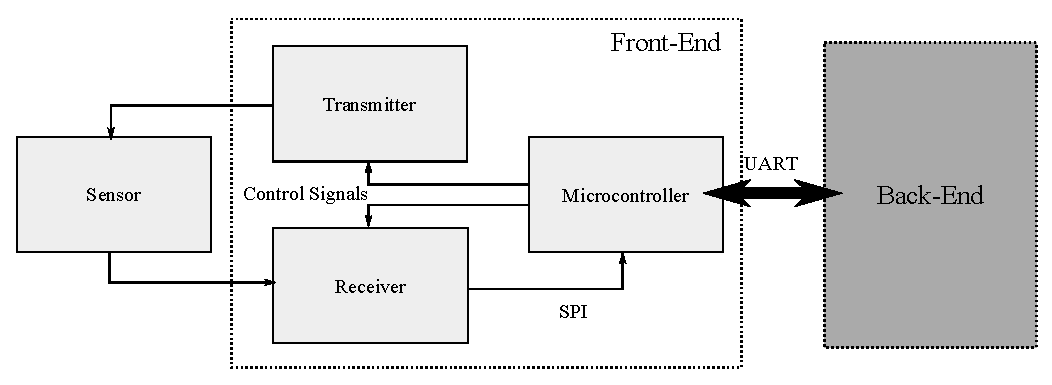
\includegraphics[scale=0.8]{kuvat/ASSP_block_diagram.eps}
  \caption{The block diagram of the new system. The system doesn't take any stand on the selection of the back-end processor -- it can be a microcontroller, a DSP or even a PC.}
  \label{fig:ASSP_block_diagram}
\end{figure}

\subsection{Microcontroller}

The microcontroller used is TI MSP430F5529 \cite{MSP430F5529}, an ultra-low power RISC processor with a number of peripheral modules. The processor is in the higher end of the MSP430 family with several DMA channels, four timers and many communication modules, yet still doesn't have the processing power of e.g. ARM processors. It is still powerful enough to perform well as a measurement module for a host processor or even as a stand-alone unit with a less advanced signal processing algorithm using only a minimal amount of electrical power.

In addition to a number of general purpose I/O ports and a USB module, the microcontroller has two USCI modules for communicating with a host processor or other peripherals. One of them is dedicated for communicating with the AFE's analog-to-digital converter via SPI. In the developed application the other one is used for host communication via UART yet possible other solutions include, but aren't limited to, operating a display driver for displaying results or sending the measurement data using an external radio module.

\subsection{Analog Front-End}

The analog front-end consists of a current-regulating transmitter, a receiver with multiple gain stages and a 22-bit ADC. It is capable of performing hardware diagnostic tests on the probe, checking for short and open circuits on all the lead combinations. It supports two transmit channels and four measurements per cycle, measuring both the ``LED ON'' value and the ambient value for both channels. LED current and receiver gain are individually selectable for both channels, enabling truly independent control for both of them.

The key to the operation of the AFE is timing. A number of control signals are produced for all the components of the AFE, guiding their operation precisely. The signals are ``enabling'' signals as opposed to triggering signals: For example, from the internal timer's perspective the signal \textit{RED ON} is defined as the interval between a starting counter value and an ending counter value and is set high for that period of time. It is then used so that current is fed into the red LED when said signal is high. The same applies for other timing signals (LED ON, SAMPLE, CONVERT). It's up to the microcontroller software to set the compare registers' values so that the possibly conflicting signals don't overlap.

%\begin{figure}[htcb]
%\centergraphics{kuvat/timer_compare_register.eps}
%\caption{A timer compare module: the two register compare matches, START and STOP, set and reset the output signal.}
%\label{fig:timer_compare_register}
%\end{figure}

The transmitter (figure \ref{fig:transmitter_afe}) has two active parts: a current controller that gets its reference from an 8-bit D/A converter, and an H-bridge for switching the current on and off for each LED in configurations shown in figure \ref{fig:led_configurations}. In short, it provides precisely timed pulses with constant currents without any crosstalk between the two channels. As the power supply is current limited and the drive capacitor not infinite the pulses have to be separated enough, though, or otherwise the latter might suffer from the temporary voltage drop caused by the former when using high LED currents.

\begin{figure}[htcb]
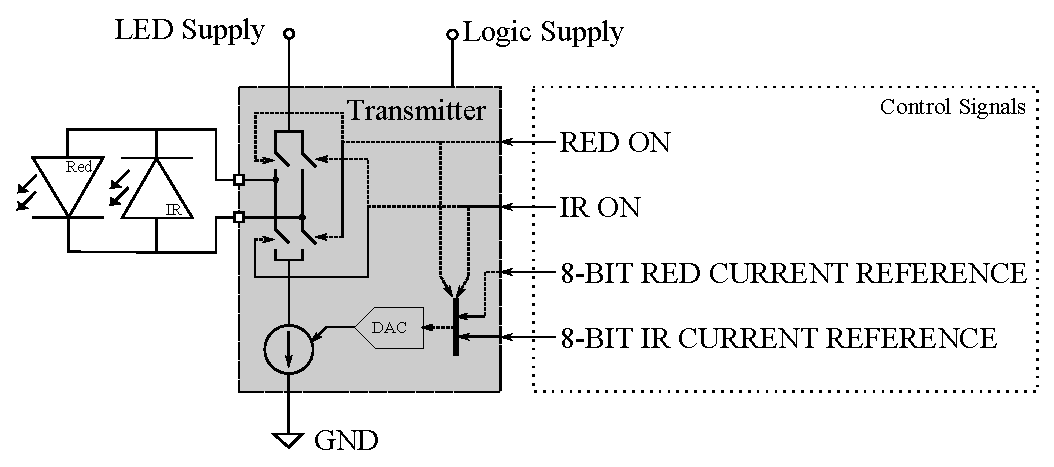
\includegraphics[scale=0.75]{kuvat/transmitter_afe.eps}
\caption{A block diagram of the AFE's transmitter unit showing the H-bridge, the current controller and the control signals.}
\label{fig:transmitter_afe}
\end{figure}

The receiver is a bit more complicated (figure \ref{fig:receiver_afe}), consisting of an amplifier with selectable gain and filtering properties, four sampling units and a buffered A/D converter. The gain can be set by selecting a value for the feedback resistor R\subscript{f} out of the values available, ranging from 10 k$\Omega$ to 1 M$\Omega$. The amplifier's time constant and thus its low-pass bandwidth is defined by the combination of R\subscript{f} and the feedback capacitor C\subscript{f}, implying that the two should be defined as pairs. The cutoff frequency is also coupled with the LED pulse length: the shorter the pulse the higher the amplifier's bandwidth must be. This imposes another optimization problem since energy-and-signal-strength-wise a shorter pulse with a higher amplitude is preferred to a longer pulse with a lower one, but increasing the filter bandwidth to allow the shorter pulse also increases the relative amount of noise passed through.

\begin{figure}[htcb]
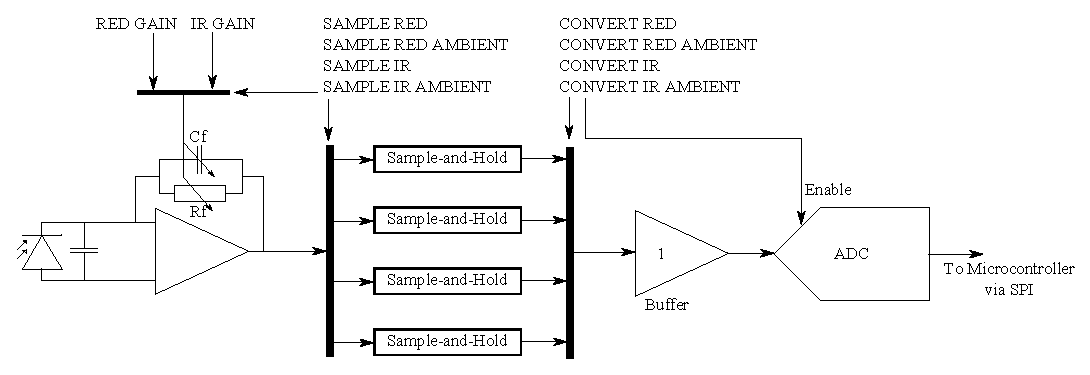
\includegraphics[scale=0.8]{kuvat/receiver_afe.eps}
\caption{A block diagram of the AFE's receiver unit, showing how the various signals control its operation.}
\label{fig:receiver_afe}
\end{figure}

\subsection{Advantages and Drawbacks}

The most obvious advantage of the setup is its reduced power consumption since it's the first GE design to specifically take that into account. By implementing the measurement control with a low-power microcontroller and buffering the samples the back-end processor can remain in sleep mode for most of the time, only waking up to handle new measurements; also designing the system with power consumption in mind from the beginning allows for a more optimized design. The power used for front-end processing alone can be reduced to 1 mW and the power used by the AFE, excluding LED drive power, is in the range of 6 mW. Compared to the average power consumption of a suitable ARM microcontroller (Atmel SAM3S, 90mW) \cite{ATMEL2009}, not to mention a conventional AFE, the power reduction is significant.

The other major upside in the design is its mechanical simplicity: in addition to being small, once the module is completed it will be extremely easy to design a range of platforms with different peripherals for it. Also the assembly process is simpler and cheaper due to the reduced number of components. In short, the design allows for a device that is more power-efficient and in many cases cheaper to manufacture without compromising the accuracy of the measurement.

A drawback in the solution is that it leaves little room for future development as it is heavily optimized for current design specifications. Therefore scaling it up for more wavelengths or more processing power is out of the question without significant existing market demand.

\subsection{Special Considerations for Verification}

The special design of this chip makes its verification process and performance tests a bit more difficult than usual: as the circuitry is very tightly packed and well shielded it is practically impossible to measure signals within the receiver chain without affecting performance. This calls for a new statistical approach for assessing performance, a kind of regression analysis, which is the main emphasis of this thesis and will be thoroughly explained in sections \ref{section:prototype_validation} and \ref{section:performance_analysis}.